\documentclass[twoside]{article}

%\usepackage{aistats2019}
% If your paper is accepted, change the options for the package
% aistats2019 as follows:
%
\usepackage[]{aistats2019}

\usepackage{graphicx}
\usepackage{subfigure}
%
% This option will print headings for the title of your paper and
% headings for the authors names, plus a copyright note at the end of
% the first column of the first page.

% If you set papersize explicitly, activate the following three lines:
%\special{papersize = 8.5in, 11in}
%\setlength{\pdfpageheight}{11in}
%\setlength{\pdfpagewidth}{8.5in}

% If you use natbib package, activate the following three lines:
% \usepackage[round]{natbib}
% \renewcommand{\bibname}{References}
% \renewcommand{\bibsection}{\subsubsection*{\bibname}}

\usepackage[style=numeric-comp,
            sorting=none,
            backend=bibtex,
            maxnames=2,
            maxbibnames=99]{biblatex}
\bibliography{main.bib}


% If you use BibTeX in apalike style, activate the following line:
%\bibliographystyle{apalike}
% Attempt to make hyperref and algorithmic work together better:
\usepackage{hyperref}       % hyperlinks
\usepackage{url} 
\usepackage{booktabs} 
\usepackage{nicefrac} 
\usepackage{algorithm}
\usepackage{algorithmicx}
\usepackage[noend]{algpseudocode}
%\usepackage[square,numbers]{natbib}   
\usepackage{subcaption}
\usepackage{array}
\usepackage{float}
\usepackage{amsmath}
\usepackage{amssymb}
\usepackage{amsfonts}
\usepackage{latexsym}
\renewcommand{\algorithmicrequire}{\textbf{Input:}}
\renewcommand{\algorithmicensure}{\textbf{Output:}}

\algnewcommand\algorithmicassert{\texttt{assert}}
\algnewcommand\Assert[1]{\State{} \algorithmicassert(#1)}

\algnewcommand\algorithmicswitch{\textbf{switch}}
\algnewcommand\algorithmiccase{\textbf{case}}
\algnewcommand\algorithmicdefault{\textbf{default}}
\algdef{SE}[SWITCH]{Switch}{EndSwitch}[1]{\algorithmicswitch\ #1\ \algorithmicdo}{\algorithmicend\ \algorithmicswitch}
\algdef{SE}[CASE]{Case}{EndCase}[1]{\algorithmiccase\ #1}{\algorithmicend\ \algorithmiccase}
\algdef{SE}[DEFAULT]{Default}{EndDefault}[1]{\algorithmicdefault\ #1}{\algorithmicend\ \algorithmicdefault}
\algtext*{EndSwitch}
\algtext*{EndCase}
\algtext*{EndDefault}

\algnewcommand\algorithmicmatch{\textbf{match}}
\algdef{SE}[MATCH]{Match}{EndMatch}[1]{\algorithmicmatch\ #1}{\algorithmicend\ \algorithmicmatch}
\algtext*{EndMatch}

\algnewcommand\algorithmictry{\textbf{try}}
\algnewcommand\algorithmiccatch{\textbf{catch}}
\algblockdefx[Try]{Try}{EndTry}{\algorithmictry}{\algorithmicend\ \algorithmictry}
\algtext*{EndTry}
\algcblockdefx[Catch]{Try}{Catch}{EndTry}[1]{\algorithmiccatch\ #1}{\algorithmicend\ \algorithmictry}%
\algtext*{EndTry}
\MakeRobust{\Call}

\algdef{SE}[QUERY]{Query}{EndQuery}%
   [2]{\textbf{query}\ \textproc{#1}\ifthenelse{\equal{#2}{}}{}{(#2)}}%
   {\algorithmicend\ \algorithmicquery}%
\algtext*{EndQuery}

\def\@algocf@capt@ruled{under}



\newcommand{\theHalgorithm}{\arabic{algorithm}}


\newcommand{\SL}{\mathcal{S}}  % set of start locations
\newcommand{\GL}{\mathcal{G}}  % set of goal locations

\newcommand{\C}{{C}}  % chaser variables
\newcommand{\R}{{R}}  % runner variables

\newcommand{\cs}{\C_s} % chaser start

\newcommand{\cg}{\C_g} % chaser goal
\newcommand{\cp}{\C_p} % chaser path

\newcommand{\rs}{\R_s} % runner start
\newcommand{\rg}{\R_g} % runner goal
\newcommand{\rp}{\R_p} % runner path

\newcommand{\obs}{o} % observations

\newcommand{\crs}{x^\textsc{r}_\textsc{start}} % chaser thinks runner start
\newcommand{\crg}{x^\textsc{r}_\textsc{goal}} % chaser thinks runner goal
\newcommand{\crp}{x^\textsc{r}_{1:T}} % chaser thinks runner path

\newcommand{\rcs}{\tilde{x}^\textsc{c}_\textsc{start}} % runner thinks chaser start
\newcommand{\rcg}{\tilde{x}^\textsc{c}_\textsc{goal}} % runner thinks chaser goal
\newcommand{\rcp}{\tilde{x}^\textsc{c}_{1:T}} % runner thinks chaser path


\newcommand{\rdet}{\R_{\delta}} % runner detection
\newcommand{\cdet}{\C_{\delta}} % runner detection


\renewcommand{\det}{\delta} % detection

\newcommand{\dprob}{\beta} % detection probability
\newcommand{\rdprob}{\C_\beta} % chaser's detection probability
\newcommand{\cdprob}{\R_\beta} % runner's detection probability


\newcommand{\cat}{\mathrm{Cat}}  % categorical
\newcommand{\nor}{\mathcal{N}}  % normal
\newcommand{\ber}{\mathrm{Ber}}  % normal

\newcommand{\rrt}{\mathrm{RRT}}  % maybe \optim_rrt? rrt
\newcommand{\query}{\mathrm{query}}

\newcommand{\innermost}{\mathcal{I}}
\newcommand{\middlemost}{\mathcal{M}}
\newcommand{\outermost}{\mathcal{O}}

\newcommand{\isovist}{\mathrm{isovist}}

\newcommand{\qry}{\ensuremath{$\reflectbox{$\,\leadsto$}$}}

\begin{document}

% If your paper is accepted and the title of your paper is very long,
% the style will print as headings an error message. Use the following
% command to supply a shorter title of your paper so that it can be
% used as headings.
%
%\runningtitle{I use this title instead because the last one was very long}

% If your paper is accepted and the number of authors is large, the
% style will print as headings an error message. Use the following
% command to supply a shorter version of the authors names so that
% they can be used as headings (for example, use only the surnames)
%
%\runningauthor{Surname 1, Surname 2, Surname 3, ...., Surname n}


\twocolumn[

\aistatstitle{Modeling Theory of Mind for Autonomous Agents\\ with Probabilistic Programs}

\aistatsauthor{ Iris R. Seaman \And  Jan-Willem van de Meent \And David Wingate}

\aistatsaddress{ seaman.i@northeastern.edu \And j.vandemeent@northeastern.edu \And wingated@cs.byu.edu} ]

\begin{abstract}
As autonomous agents
become more ubiquitous, they will eventually have to reason about the mental state of
other agents, including those agents' beliefs, desires and goals --
so-called \emph{theory of mind} reasoning. We introduce a collection of increasingly complex theory of mind models of a ``chaser'' pursuing a ``runner'', known as the \textit{Chaser-Runner} model. We show that our implementation is a relatively straightforward theory of mind model that can capture a variety of rich behaviors, which in turn, increase runner detection rates relative to basic (non-theory-of-mind) models. In addition, our paper demonstrates that (1) using a planning-as-inference formulation based on nested importance sampling results in agents simultaneously reasoning about other agents' plans and crafting counter-plans, (2) probabilistic programming is a natural way to describe models in which each uses complex primitives such as path planners to make decisions, and (3) allocating additional computation to perform nested reasoning about agents result in lower-variance estimates of expected utility.

%As autonomous agents become more ubiquitous, they will eventually have to reason about the mental state of
% other agents, including those agents' beliefs, desires and goals --
% so-called \emph{theory of mind} reasoning.We describe increasingly complex theory of mind models of a
% ``chaser'' pursuing a ``runner'' and show that (1) there is a natural
% probabilistic formulation to reasoning about the uncertainty 
% in our estimate of another agent's mental state, and that (2)
% probabilistic programming is a natural way to describe models 
% in which each uses complex primitives such as path planners 
% to make decisions. We use a planning-as-inference formulation based on 
% nested importance sampling to simultaneously reason about other agents' 
% plans and craft counter-plans, and quantify the trade-offs in allocating 
% our sample budget at different levels of the model.
\end{abstract}

% --------------------------------------------------------------------------------
\vspace{-2.0em}
\section{Introduction}
\label{sec:intro}
\vspace{-0.75em}

% As autonomous agents (such as unmanned aerial vehicles, or UAVs) become more ubiquitous, they are being used for increasingly complex tasks. 
An autonomous agent that interacts with other agents needs to do more than simply perceive and respond to their environment. 
Eventually agents will need to reason about all of
the complexities inherent in the real world, including 
the beliefs, intents and desires of other intentional agents.  This is
known as \textit{theory of mind}, and is indispensable if we hope to
one day create agents capable of empathy, ``reading between the
lines,'' and interacting with humans as peers. %Fortunately, many of
%the needed pieces already exist in the intersection between control
%theory and machine learning.

In this paper, we explore how theory of mind can be implemented using 
nested simulations in the form of probabilistic programs.
We develop a scenario involving two agents, a \textit{chaser} and
a \textit{runner}. %We begin with the basic idea that t
The chaser seeks to intercept the runner and the runner seeks to reach a goal location without
detection. However, the runner's intended start location, goal
location, and likely path to the goal are initially unknown to the
chaser. We assume that the runner knows the current location of the 
chaser, but not where the chaser will move in the future. This results in a setting where both agents must reason about each other, and about how they reason about reasoning.

% 1) Regular SMC problem has been done before for probabilistic programming
% -----> extrememly limited, no Time 
% 2) Nested IS is not the same as Nested MC (problem is language here)


%In this paper, our goal is to take a step towards a framework that
%could actually be deployed on a real UAV.

To simulate runner and chaser trajectories, we employ a 
variety of semi-realistic primitives, including path planners and 
visibility graphs. 
%We formulate the model of the chaser and the runner as nested probabilistic programs, which are conditioned to \emph{maximize} the likelihood of detection from the perspective of the chaser model, and \emph{minimize} likelihood of detection from the perspective of the runner model.
%
We formulate the model of the chaser and the runner
as nested probabilistic programs, which are conditioned according to the desired behavior of the respective agents. The model of the chaser is conditioned to 
\emph{maximize} the likelihood of detection, and the runner is conditioned to \emph{minimize} likelihood of detection.
%
The result is a probabilistic model over possible chaser trajectories. At each point of time, the chaser imagines 
possible future trajectories, along with possible runner trajectories, and selects 
a move that has a high relative expected utility. This planning-as-inference 
formulation \cite{toussaint06} is a natural fit for probabilistic programming, 
which makes it straightforward to incorporate complex deterministic primitives 
into both models, and perform recursive Bayesian reasoning using the framework 
of nested importance sampling \cite{naesseth2015nested}.

We evaluate our models in a variety of scenarios and demonstrate that nested Bayesian reasoning leads to rational behaviors which maximize utility respectively at each level. Our experiments show that our formulation leads to improved runner detection rates relative to basic models, and that allocating additional computation to perform nested reasoning about agents results in lower-variance estimates of expected utility. 


%-------------------

%---------------------

% --------------------------------------------------------------------------------


\begin{figure*}
\begin{center}
\vspace{-1.0em}
\centerline{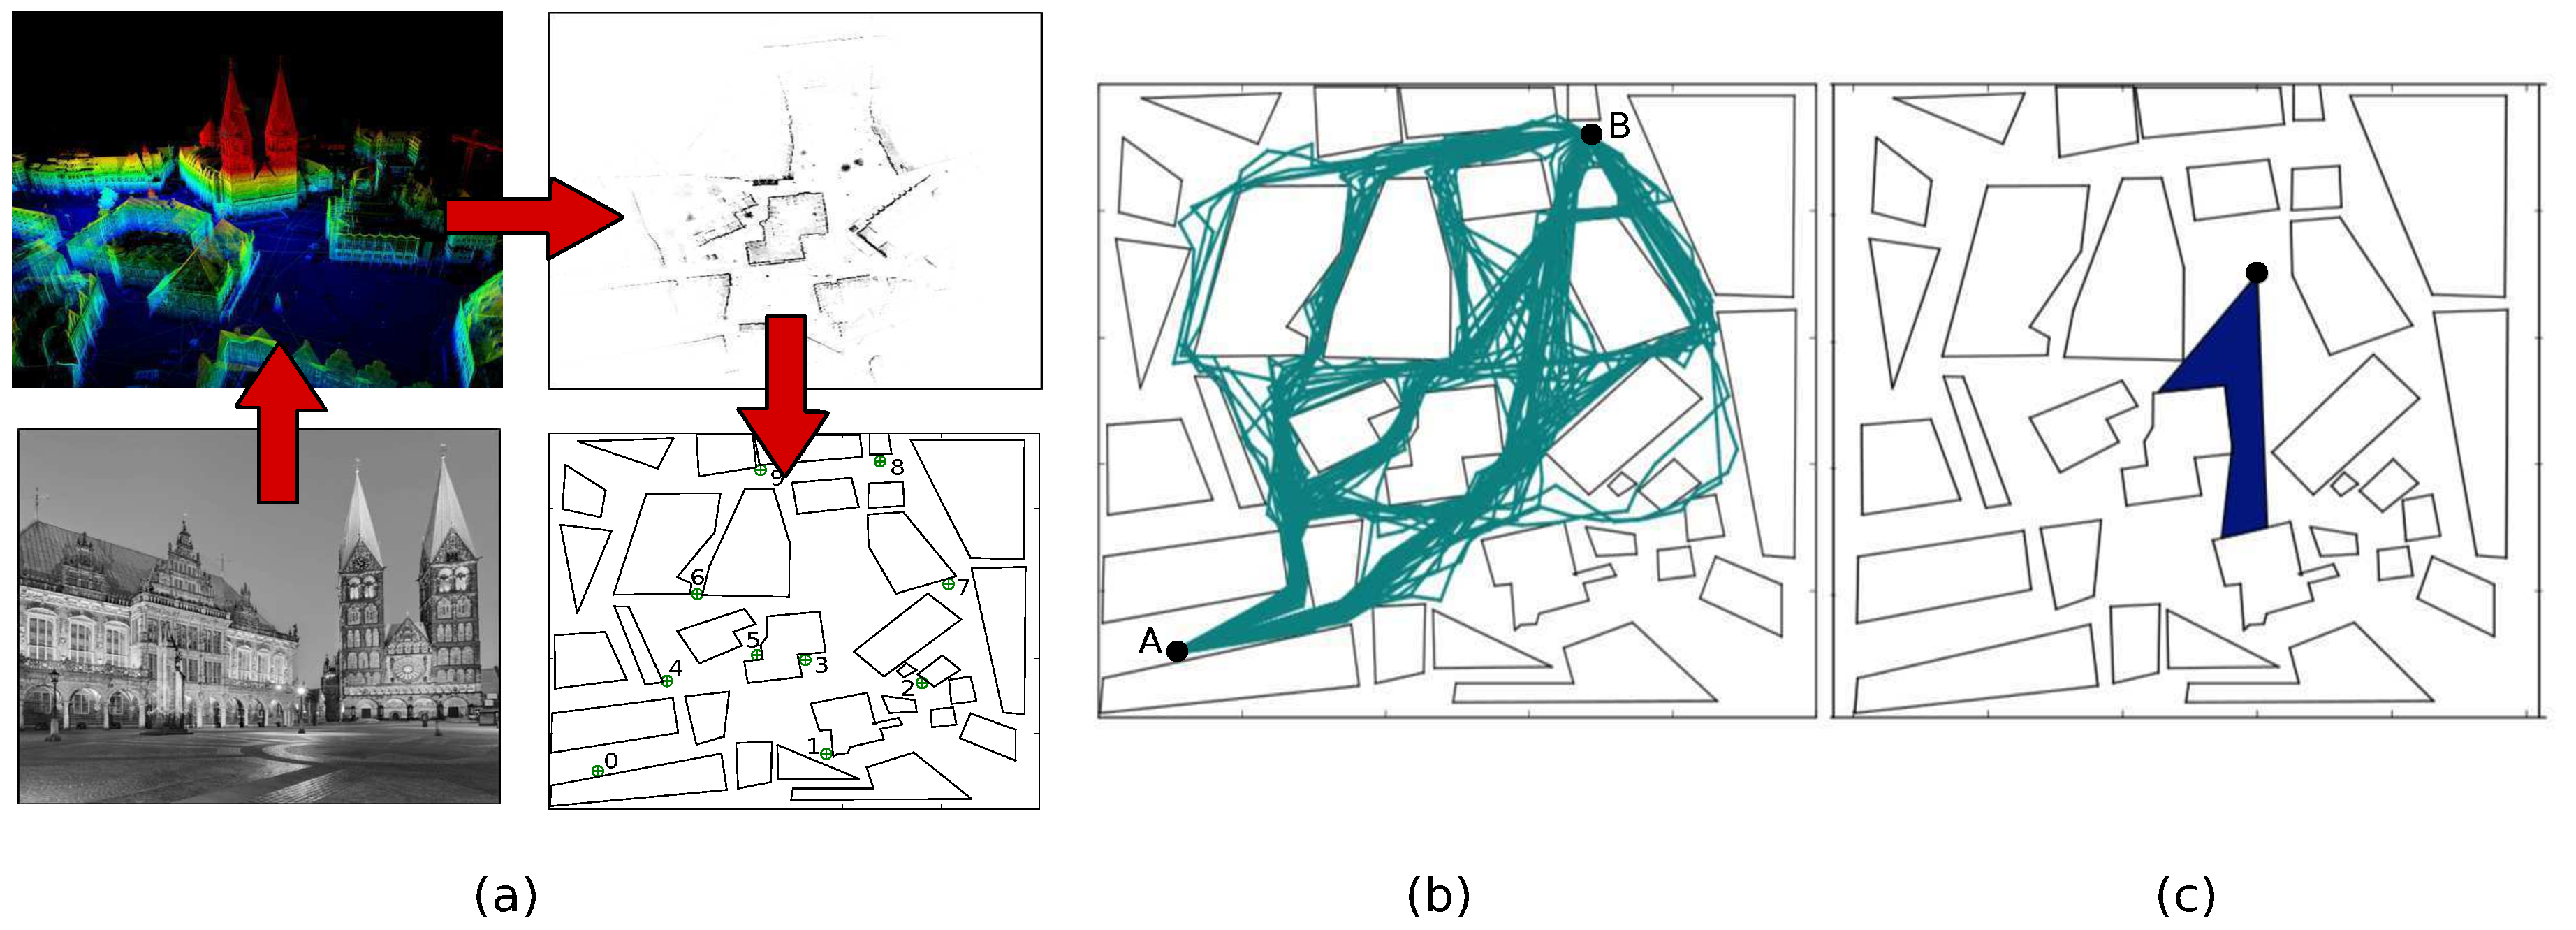
\includegraphics[width=0.9\textwidth]{sim_primitives.eps}}
\caption{(a) We generate a coarse polygonal city map from point cloud data of the city of Bremen, Germany. (b) Visual distribution over paths a runner may take
modeled with Random-Exploring Random Trees, RRTs, from points A to B. (c) a 45$^{\circ}$ isovist, or range of sight, of the
chaser.  The isovist is properly blocked by buildings.}
\label{fig:rrt}
\end{center}
\vspace{-1.0em}
\end{figure*} 

\section{Background}

\subsection{Theory of Mind}

Human children develop theory of mind during their
early years, generally between the ages of three and
six
\cite{wellman1990child,chater2006probabilistic}. \textcite{bello2006developmental}
explore this phenomenon with a computational model that suggests that the underlying cognitive shifts required for the development of theory of mind may be smaller than previously supposed. 
%
\textcite{goodman2006intuitive} present a formal model that
attempts to account for false belief in
children, and later take the innovative approach of
linking inference with causal reasoning \cite{goodman2009cause}. Additionally, the same group explores language as a type of social
cognition \cite{goodman2013knowledge}.
%

The development of theory of mind in machines leads naturally to interaction with their human counterparts. \textcite{awais2010human}, \textcite{fern2007decision}, and \textcite{nguyen2012capir} investigate collaboration between humans and robots in which the robot must determine the human's (unobservable) goal. In a complementary line of research, \textcite{sadigh2016information} explore the idea of active information, in which the agent's own behaviors become a tool for identifying a human's internal state.

Fully-developed theory of mind requires the possibility of nested beliefs. \textcite{koller1997effective} present an inference algorithm for recursive stochastic programs. \textcite{frith2005theory} argue that theory of mind can be modeled using probabilistic programming, and demonstrate examples of nested conditioning with the probabilistic programming language, Church. \textcite{zettlemoyer2009multi} address filtering in environments with many agents and infinitely nested beliefs. 

There has thus far been comparatively little work on modeling theory of mind in a time-dependent manner. 
\textcite{baker2009action} develop a computational framework based on action understanding as inverse planning. Similar to this work, we limit our study to a single agent reasoning about another agent. Our work differs in that our environment is not discretized into a grid world, and as such represents a continuous environment and action space, which is supported by random planning of Rapidly-Exploring Random Trees (RRTs) for decision making. More recently, \textcite{stuhlmuller2014reasoning} emphasized the value of probabilistic programs in modeling the reasoning of other agents. We build upon this work by modeling theory of mind in a more temporal setting, where agents must update and \textit{act upon} their beliefs of other agents.

% Fully-developed theory of mind requires the possibility of nested beliefs. \textcite{zettlemoyer2009multi} address filtering in environments with many agents and infinitely nested beliefs. \textcite{koller1997effective} present an inference algorithm for recursive stochastic programs, while \textcite{baker2009action} present a computational framework based on action understanding as inverse planning. More recently, \textcite{stuhlmuller2014reasoning} emphasized the value of probabilistic programs in modeling the reasoning of other agents. Finally, \textcite{frith2005theory} argue that theory of mind can be approximately represented using probabilistic programming, and demonstrate examples of nested conditioning with the probabilistic programming language, Church.



%\vspace{-0.6em}
\subsection{Probabilistic Program Inference}

To represent our generative model cleanly and to perform inference in it, we employ the tools of probabilistic programming \cite{vandemeent2018introduction}. This allows us to define probabilistic models that incorporate recursion, libraries of deterministic primitives, and data structures. %Example languages include Venture~\cite{mansinghka2014venture}, Anglican~\cite{tolpin2016design}, and Church~\cite{goodman08}.
A probabilistic program is a procedural model that, when run unconditionally, yields a sample from a prior distribution. Running probabilistic programs forward can be quite fast, and is limited only by the native speed of the interpreter for the language.

Inference in probabilistic programming involves reasoning about a target distribution that is conditioned by a likelihood, or more generally a notion of utility \cite{vandemeent2018introduction}.
Inference for probabilistic programs is difficult because of the flexibility that probabilistic programming languages provide: an inference algorithm must behave reasonably for any program a user wishes to write. Many probabilistic programming systems rely on Monte Carlo methods due to their generality \cite{goodman08,milch05,pfeffer01,standevelopmentteam2014stan,venture}. Methods based on importance sampling and SMC have become particularly popular \cite{murray2013,todeschini2014biips,wood-aistats-2014,goodman2014dippl,ge2016turing}, owing to their simplicity and compositionality \cite{naesseth2015nested}.

For our purposes, the most important feature of probabilistic programming languages is that they allow programmers to freely mix deterministic and stochastic elements, resulting in tremendous modeling flexibility.  This makes it relatively easy to (for example) describe distributions over Rapidly-Exploring Random Tree (RRTs), isovists, or even distributions that involve optimization problems as a subcomponent of the distribution.

% --------------------------------------------------------------------------------
% --------------------------------------------------------------------------------
% --------------------------------------------------------------------------------


\section{Simulation Primitives}
%\vspace{-0.5em}

Although probabilistic programming has previously been used to model theory of mind \cite{baker2009action, stuhlmuller2014reasoning}, past implementations have thus far considered relatively simplistic settings. In this paper we not only model a setting in which agents must reason about future events, but also do so in a manner that involves reasoning about properties of the physical world around them. To enable this type of reasoning, we will employ a number of semi-realistic simulation primitives.

\textbf{The environment.}  To search for and intercept the runner, the
chaser requires a representation of the world that allows reasoning
about starting locations, goals, plans, movement and visibility. We
use a polygonal model designed around a known, fixed map of the city of
Bremen, Germany \cite{BremenPointCloud}, shown in Fig.~\ref{fig:rrt} (a).

\textbf{Path planning and trajectory optimization.}  We model paths
using a RRT
\cite{lavalle1998rapidly}, a randomized path planning algorithm
designed to handle nonholonomic constraints and high degrees of
freedom.  We leverage the random nature of the RRT to describe an
entire distribution over possible paths: each generated RRT path can
be viewed as a sample from the distribution of possible paths taken by
a runner (see Fig.~\ref{fig:rrt} (b)). RRTs naturally consider short
paths as well as long paths to the goal location. To foreshadow a bit,
note that because we will be performing inference over RRTs
conditioned on not being detected, the runner will naturally tend to
use paths that minimize the chance of detection, which are often, but
not always, the shortest and most direct.  Our RRTs are
refined using a trajectory optimizer to eliminate bumps
and wiggles.

\textbf{Visibility and detection.}  Detection of the runner by the
chaser is modeled using an isovist, a polygon
representation of the chaser's current range of sight
\cite{isovist79,morariu2007human}. Given a map, chaser location, and
runner location, the isovist determines the likelihood
that the runner was detected. Although an isovist usually uses a 360
degree view to describe all possible points of sight to the chaser, we
limit the range of sight to 45
degrees, and add direction to the chaser's sight as seen in
Fig.~\ref{fig:rrt} (c). The direction of the chaser's line of sight is determined by the imagined location of the runner.

% --------------------------------------------------------------------------------
% --------------------------------------------------------------------------------
% --------------------------------------------------------------------------------

%\vspace{-0.5em}
\section{The Chaser-Runner Model}
%\vspace{-0.5em}


\label{sec:tcrm}

Here we describe the centerpiece of our paper, the \emph{Chaser-Runner model}.  We will primarily describe this model from the perspective
of the chaser; the runner model differs from the chaser model in that
the runner wishes to minimize the probability of detection, whereas the chaser wishes to maximize it.
Our model has four levels: the \textbf{episode model} samples a sequence of moves by the chaser. Each move is sampled from the \textbf{outermost model}, which describes the
beliefs of the chaser about the expected utility of moves. This model compares future chaser trajectories to possible runner trajectories and assigns higher probability to trajectories in which the runner is likely to be detected. The runner trajectories are in turn sampled from the  \textbf{middlemost model}, which minimizes detection probability based on imagined chaser trajectories that are sampled from the \textbf{innermost model}.
%
These three models work in tandem to create nuanced inferences about
where the chaser believes the runner might be, and how it ought to 
counter-plan to maximize probability of detection.


\begin{algorithm}[!t]
\begin{algorithmic}
%\State $Q^\textsc{chaser} \gets \textbf{importance}(\textsc{chaser}, 1)$
\State $Q^\textsc{chaser} \!\gets\! \textbf{resample}(\textbf{importance}(\textsc{chaser}, K), K)$
\State $Q^\textsc{runner} \!\gets\! \textbf{importance}(\textsc{runner}, L)$
\State $Q^\textsc{naive-chaser} \!\gets\! \textbf{importance}(\textsc{naive-chaser}, 1)$
% \Query{episode}{\,}
%     \State $x^\textsc{c}_\textsc{start} \sim \text{Uniform}(\{x_\textsc{a},\ldots,x_\textsc{j}\})$
%     %\State $x^\textsc{c}_{1:T}, w^\textsc{c} \sim \textbf{query}(\textsc{chaser}, x^\textsc{c}_\textsc{start}, K)$
%     \State $x^\textsc{c}_{1:T}, w^\textsc{c} \sim Q^\textsc{chaser}(x^\textsc{c}_\textsc{start})$    
%     \State \Return $x^\textsc{c}_{1:T}, w^\textsc{c}$
% \EndQuery
\Query{episode}{$x^\textsc{c}_\textsc{start}$}
    \Comment{Episode model}
    \State $x^\textsc{c}_1 \gets x^\textsc{c}_\textsc{start}$
    \For{$t$ \textbf{in} $2 \ldots T$}
    %\State $x^\textsc{c}_t, w_t^\textsc{c} \sim \textbf{`y}(\textsc{chaser}, x^\textsc{c}_{1:t-1}, L)$
    \State $x^\textsc{c}_{1:t}, w_t \qry Q^\textsc{chaser}(x^\textsc{c}_{1:t-1})$    
    \EndFor
    \State \Return $x^\textsc{c}_{1:T}, \prod_t w_t$
\EndQuery
\Query{chaser}{$x^\textsc{c}_{1:t-1}$}
    \Comment{Outer Model}
    \State $x^\textsc{c}_\textsc{goal} \sim \text{Uniform}(\{x_\textsc{a},\ldots,x_\textsc{j}\})$
    \State $x^\textsc{c}_{t:T} \sim \Call{rrt-plan}{x^\textsc{c}_{t-1}, x^\textsc{c}_\textsc{goal}}$
    %\State $x^\textsc{r}_{t+1:T}, w^\textsc{r} \sim \textbf{query}(\textsc{runner}, x^\textsc{c}_{1:t}, M)$
    \State $x^\textsc{r}_{t:T}, w^\textsc{r} \qry Q^\textsc{runner}(x^\textsc{c}_{1:t-1})$
    \State $T^\textsc{c}_\textsc{visible} \gets \Call{time-visible}{x^\textsc{r}_{t:T}, x^\textsc{c}_{t:T}}$
    %\State $w^\textsc{d} \gets \exp(\alpha T^\textsc{c}_\textsc{visible})$
    %(1-\mu)^{T-T^\textsc{c}_\textsc{visible}}$
    \State $w^\textsc{c} \gets \exp(\alpha \; T^\textsc{c}_\textsc{visible})$
    \State \Return $x^\textsc{c}_{1:t}, w^\textsc{c} \cdot w^\textsc{r}$
\EndQuery
\Query{runner}{$x^\textsc{c}_{1:t-1}$} \Comment{Middle Model}
    \State $x^\textsc{r}_\textsc{start} \sim \text{Uniform}(\{x_\textsc{a},\ldots,x_\textsc{j}\})$
    \State $x^\textsc{r}_\textsc{goal} \sim \text{Uniform}(\{x_\textsc{a},\ldots,x_\textsc{j}\})$
    \State $x^\textsc{r}_{1:T} \sim \Call{rrt-plan}{x^\textsc{r}_\textsc{start}, x^\textsc{r}_\textsc{goal}}$
    %\State $w^\textsc{d}_{\textsc{p}} \gets \exp \left( - \alpha^\textsc{r}_\textsc{p} \cdot \Call{num-detect}{x^\textsc{c}_\textsc{1:t}, x^\textsc{c}_{1:t}}  \right)$
    \State $\tilde{x}^\textsc{c}_{t:T}, \tilde{w}^\textsc{c} \qry Q^\textsc{naive-chaser}(x^\textsc{c}_{t-1})$
    \State $T^\textsc{r}_\textsc{visible} \gets \Call{time-visible}{x^\textsc{r}_{1:T}, \{x^\textsc{c}_{1:t-1}, \tilde{x}^\textsc{c}_{t:T}\}}$
    \State $w^\textsc{r} \gets \exp(-\alpha \; T^\textsc{r}_\textsc{visible})$
    \State \Return $x^\textsc{r}_{t:T},  w^\textsc{r} \cdot \tilde{w}^\textsc{c}$
\EndQuery
\Query{naive-chaser}{$x^\textsc{c}_{t-1}$} \Comment{Inner Model}
    \State $\tilde{x}^\textsc{c}_\textsc{goal} \sim \text{Uniform}(\{x_\textsc{a},\ldots,x_\textsc{j}\})$
    \State $\tilde{x}^\textsc{c}_{t:T} \sim \Call{rrt-plan}{x^\textsc{c}_{t-1}, \tilde{x}^\textsc{c}_\textsc{goal}}$ 
    \State \Return $\tilde{x}^\textsc{c}_{t:T}, 1$
\EndQuery
\end{algorithmic}

\caption{
\label{alg:chaser-runner-programs}
Probabilistic program implementation of the Chaser-Runner model. The \textsc{episode} model samples moves from a nested \textsc{chaser} model, which in turn simulates runner trajectories from a second nested \textsc{runner} model. The \textsc{chaser} model is conditioned to \emph{maximize} the probability of future detections, whereas the \textsc{runner} model is conditioned \emph{minimize} both past and future detections. At each time step $t$, we propose $K$ future trajectories for the chaser and $K \times L$ trajectories for the runner. These trajectories are then resampled to $K$ partial trajectories $x^\textsc{c}_{1:t}$, resulting in a SMC sampler for the \textsc{chaser} model.}
% \label{alg:genproc}
\end{algorithm}

Algorithm~\ref{alg:chaser-runner-programs} shows pseudo-code for the Chaser-Runner model, formulated as nested probabilistic programs that we refer to as queries. Together, these programs define a planning-as-inference problem \cite{toussaint06} in which queries generate weighted samples, resulting in a nested importance sampling  \cite{naesseth2015nested} scheme that we describe in more detail below.

\textbf{The episode model} initializes the location of the chaser to a specified start location $x^\textsc{c}_1 = x^\textsc{c}_\textsc{start}$. For subsequent time points $t=2 \ldots T$, the model samples a weighted partial trajectory $(x^\textsc{c}_{1:t}, w_t)$ from the outermost \textsc{chaser} model. After the final iteration, the model returns the completed trajectory $x^\textsc{c}_{1:T}$ and the product over incremental weights $w_{1:T}$.

\textbf{The outermost model} describes the chaser's plan for trajectories, given the chaser's belief about possible runner trajectories. The chaser selects a goal location $x^\textsc{c}_\textsc{goal}$ at random and uses the RRT planner to sample a possible future trajectory $x^\textsc{c}_{t:T}$. Note that this trajectory is random, owing to the stochastic nature of the RRT algorithm. In order to evaluate the utility of this trajectory, the chaser imagines a possible runner trajectory by sampling from the middlemost \textsc{runner} model. The chaser then evaluates the utility of the trajectory by using an isovist representation to determine the number of time points $T^\textsc{c}_\textsc{visible}$ during which the runner is visible to the chaser. The chaser then conditions the sampled trajectories by defining a weight $w^\textsc{c} = \exp( \alpha \, T^\textsc{c}_\textsc{visible})$. As we will discuss below, this corresponds to assigning a utility proportional to $T^\textsc{c}_\textsc{visible}$ in a planning-as-inference formulation. The model discards most of the imagined future trajectory, keeping only the next time point $x^\textsc{c}_t$, and returns the partial trajectory $x^\textsc{c}_{1:t}$, together with a weight $w^\textsc{c} \cdot w^\textsc{r}$ that reflects the utility of the chaser and the runner.

\textbf{The middlemost model} describes the chaser's reasoning about possible runner trajectories. %We assume that the runner is aware of the chaser's location, for example because %the chaser is a UAV, which can be heard by the runner.
We assume that the chaser models a worst-case scenario where the runner is aware of the chaser's location. This could be, for example, because the runner uses a police scanner to listen in on the chaser's reported location.
Moreover, we assume that at any point in time, the episode only continues when the chaser has not yet detected the runner. Finally, we assume that the runner will seek to avoid detection by imagining a chaser trajectory, and then selecting a trajectory that will not intersect the that of the chaser. We implement these assumptions in the probabilistic program as follows. The runner model first selects a start location $x^\textsc{r}_\textsc{start}$ and goal location $x^\textsc{r}_\textsc{goal}$ at random, and then samples a random trajectory $x^\textsc{r}_{1:T}$ using the RRT planner. The runner then imagines a future chaser trajectory by selecting a goal location $\tilde{x}^\textsc{c}_\textsc{goal}$ at random and sampling $\tilde{x}^\textsc{c}_{t:T}$ from the innermost model. We then condition this sample by computing the total time of visibility $T^\textsc{r}_\textsc{visible}$, based on both the known past trajectory $x^\textsc{c}_{1:t-1}$ and the imagined future trajectory $\tilde{x}^\textsc{c}_{t:T}$ of the chaser. Finally, we assign a weight $w^\textsc{r} = \exp(-\alpha T^\textsc{r}_\textsc{visible})$, which corresponds to a negative utility (i.e.~a cost) proportional to $T^\textsc{r}_\textsc{visible}$ in the planning-as-inference formulation.

\textbf{The innermost model} describes future chaser trajectories imagined by the runner. This model is the simplest of all the models in our nested formulation. Given the previous location $x^\textsc{c}_{t-1}$ of the chaser, the runner imagines a goal location $\tilde{x}^\textsc{c}_\textsc{goal}$ at random and then uses the RRT planner to a sample a random future trajectory $\tilde{x}^\textsc{c}_{t:T}$. Since this model is not conditioned in any way, it returns weight 1.

% --------------------------------------------------------------------------------
% --------------------------------------------------------------------------------
% ------------------------------------------------------------
\section{Planning as Inference Formulation}

The Chaser-Runner model performs two levels of nested inference. At the episode level, we infer the next time point $x^\textsc{c}_t$, conditioning on expected future detections. In order to evaluate this likelihood, we simulate runner trajectories that are conditioned to avoid future detections. We implement conditioning using a planning-as-inference formulation for probabilistic programs \cite{toussaint06,vandemeent2016black-box}. 

In a planning-as-inference problem, we consider a target density $\pi(x) = \gamma(x) / Z$ that is defined in terms of an unnormalized density $\gamma(x)$, which in turn is defined in terms of prior $p(x)$ and a utility or reward $R(x)$,
\begin{equation}
    \gamma(x) = \exp(R(x)) p(x).
\end{equation}
% Here, the normalizing constant $Z = \mathbb{E}[\exp(R(x))]$ is sometimes referred to as the desirability \cite{todorov2009efficient}. 

The Chaser-Runner model in Algorithm~\ref{alg:chaser-runner-programs} defines a sequence of unnormalized densities 
\begin{align*}
    \gamma_t(x^\textsc{c}_{t:T}, \tilde{x}^\textsc{c}_{t:T}, x^\textsc{r}_{1:T})
    &=
    \exp[\alpha (T^\textsc{c}_\textsc{visible} - T^\textsc{r}_\textsc{visible} )] 
    \\
    &~~~~~~
    p(x^\textsc{c}_{t:T} | x^\textsc{c}_{t-1})
    p(\tilde{x}^\textsc{c}_{t:T} | x^\textsc{c}_{t-1})
    p(x^\textsc{r}_{1:T}).
\end{align*}
In this density, the reward $\alpha (T^\textsc{c}_\textsc{visible} - T^\textsc{r}_\textsc{visible})$ depends on the \emph{difference} between the number of time points during which the chaser expects that the runner will be visible, and the number of time points during which the runner expects to be visible based the imagined chaser trajectory (which reflects its more naive model of the chaser). In other words, the the chaser aims to identify trajectories that will result in likely detections of the runner, under the assumption that the runner will avoid trajectories where detection is likely given a naive chaser model. 

At each time we sample $x^\textsc{c}_t \sim \pi_t(x^\textsc{c}_t)$ from the marginal of this probabilistic model. To do so, we employ a nested importance sampling scheme, in which we sample $K$ particles from the \textsc{chaser} model at each $t$. For each of the $K$ samples, we draw $L$ samples from the \textsc{runner} model. We then perform resampling to select $K$ of the resulting $K \cdot L$ particles, which corresponds to performing SMC sampling within the \textsc{episode} model. Note that in the resulting nested sampling scheme, each of the $L$ samples corresponds a \emph{different} runner trajectory $x^\textsc{r}_{1:T}$, but that the reward for this trajectory is evaluated relative to the \emph{same} past $x^\textsc{c}_{1:t-1}$ and future $x^\textsc{c}_{t:T}$ trajectories for the chaser. 

To denote this sampling scheme, we define query distributions in lines 1-3 of Algorithm~\ref{alg:chaser-runner-programs}. We assume an operator \textbf{importance} that accepts a query and a number of samples $L$ and returns a transformed query $Q$ that accepts $K$ samples, and returns $K \times L$ weighted samples. We additionally assume a \textbf{resample} operation that accepts a query and a sample count $K$ and returns a new query that resamples $K$ samples from a query, down-sampling or up-sampling if necessary. 

% \vspace{-0.2in}
\section{Experimental Setup and Results}

Relative to previous approaches, this case study advances applying theory of mind models in a more realistic and complex setting for decision making. %We introduce nested theory of mind models that each use complex deterministic components such as RRT planners and field of view calculations as part of their model to plan and craft counter-plans against other agents. 
We carry out three categories of empirical experiments: 1) \textit{model flexibility}, where we demonstrate that rational behavior can be manifested by the models depending on conditioning, 2) \textit{detection rates}, which test to what extent a more accurate model of a runner enables the chaser to detect the runner most often, and 3) \textit{computational}, where we quantify the trade-offs in allocating our sample budget at different levels of the model. 

% old
% Our experiments test to what extent a more accurate model of a runner enables the chaser to detect the runner more often. We carry out 3 categories of experiments: 1) \textit{computational}, where we demonstrate that our inference algorithm empirically converges to the same distribution over trajectories as the one obtained using Metropolis Hastings,  2) \textit{model flexibility}, where we demonstrate that rational behavior is manifested by the models depending on conditioning, and 3) \textit{detection rates}, demonstrating that more complex models increase detection rates of the runner by implementing our full theory of mind chaser-runner model.


\begin{figure*}
\begin{center}
\centerline{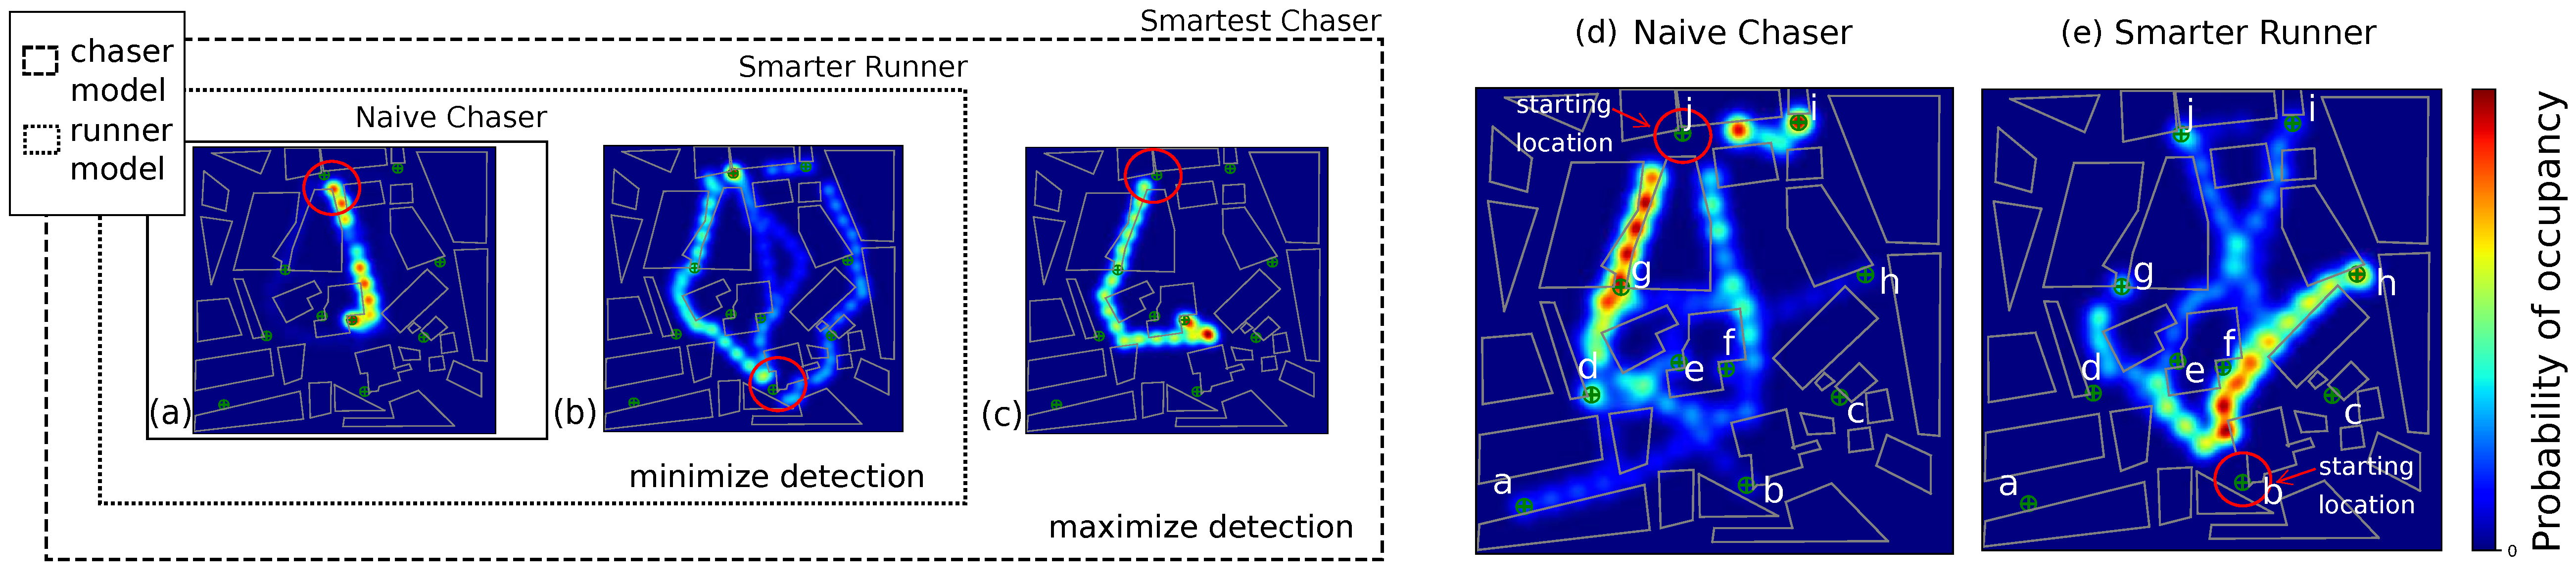
\includegraphics[width=2.0\columnwidth]{occupancy_diagram.eps}}
\caption{ \textbf{The Chaser-Runner model} showing the innermost, middlemost, and outermost models. (a)-(c) show posterior distributions over paths after running importance sampling. See text for details. Figures (d)-(e) show posterior distributions of $L$ \textit{runner} and \textit{naive chaser} paths, when $(K,L) = 128, 16$ for a single resampled $K$ sample. See text for more details. 
}
\label{fig:progression}
\end{center}
% \vskip -0.3in
\end{figure*} 


\subsection{Model Flexibility Experiments}

In these experiments, we show how nested inference converges empirically to rational behavior at each layer of the model. We begin the experiments by setting up inference to work with a worst case scenario of the runner having full knowledge of the chaser's whereabouts. %Our first experiment is shown in a series of heat maps in Figure~\ref{fig:progression} (a)-(c). 
Our first experiment begins in Figure~\ref{fig:progression} (a), with a heat map of imagined chaser paths in the innermost model where we conditioned the start and goal locations. Then we reveal how a runner, i.e. the middlemost model, uses the innermost model to plan and avoid detection while reaching the same goal as the chaser (which we in this experiment condition to be the identical), Figure~\ref{fig:progression} (b). Lastly, the outermost model converges to a plan that leads to higher detection probability of plans sampled from the middlemost model of the runner in Figure~\ref{fig:progression} (c). To this end, Figure~\ref{fig:progression} (a)-(c) demonstrates how our Chaser-Runner model can adjust planning based on simulated imagined scenarios. 

The second experiment relaxes the conditioning to observe only the start locations for each agent. We use a sample budget of $(K,L) = (128, 16)$ and view the $L$ imagined chaser and runner paths from a single $k$ sample (sampled proportionally to importance weights) in Figure~\ref{fig:progression} (d)-(e). As the runner observes the naive chaser's plans,  Figure~\ref{fig:progression} (d), the runner plans paths to maximizes utility, which tend to avoid detection from the naive chaser,  shown in Figure~\ref{fig:progression} (e). Although the naive chaser travels directly toward goal locations, in this particular $k$ sample, the naive chaser begins on the lower end of the map, therefore covering more area toward locations \textbf{b}, \textbf{c}, and \textbf{d}. This results in the runner traveling through the center of city without (or hardly any) detection.  This is a case where the RRT planner provides the runner with  a shorter and direct plan to minimize detection from the chaser. We note that for visual purposes, we display paths from time step 3 and on in Figure~\ref{fig:progression} (d)-(e). 



\begin{figure}[!t]
\begin{center}
\centerline{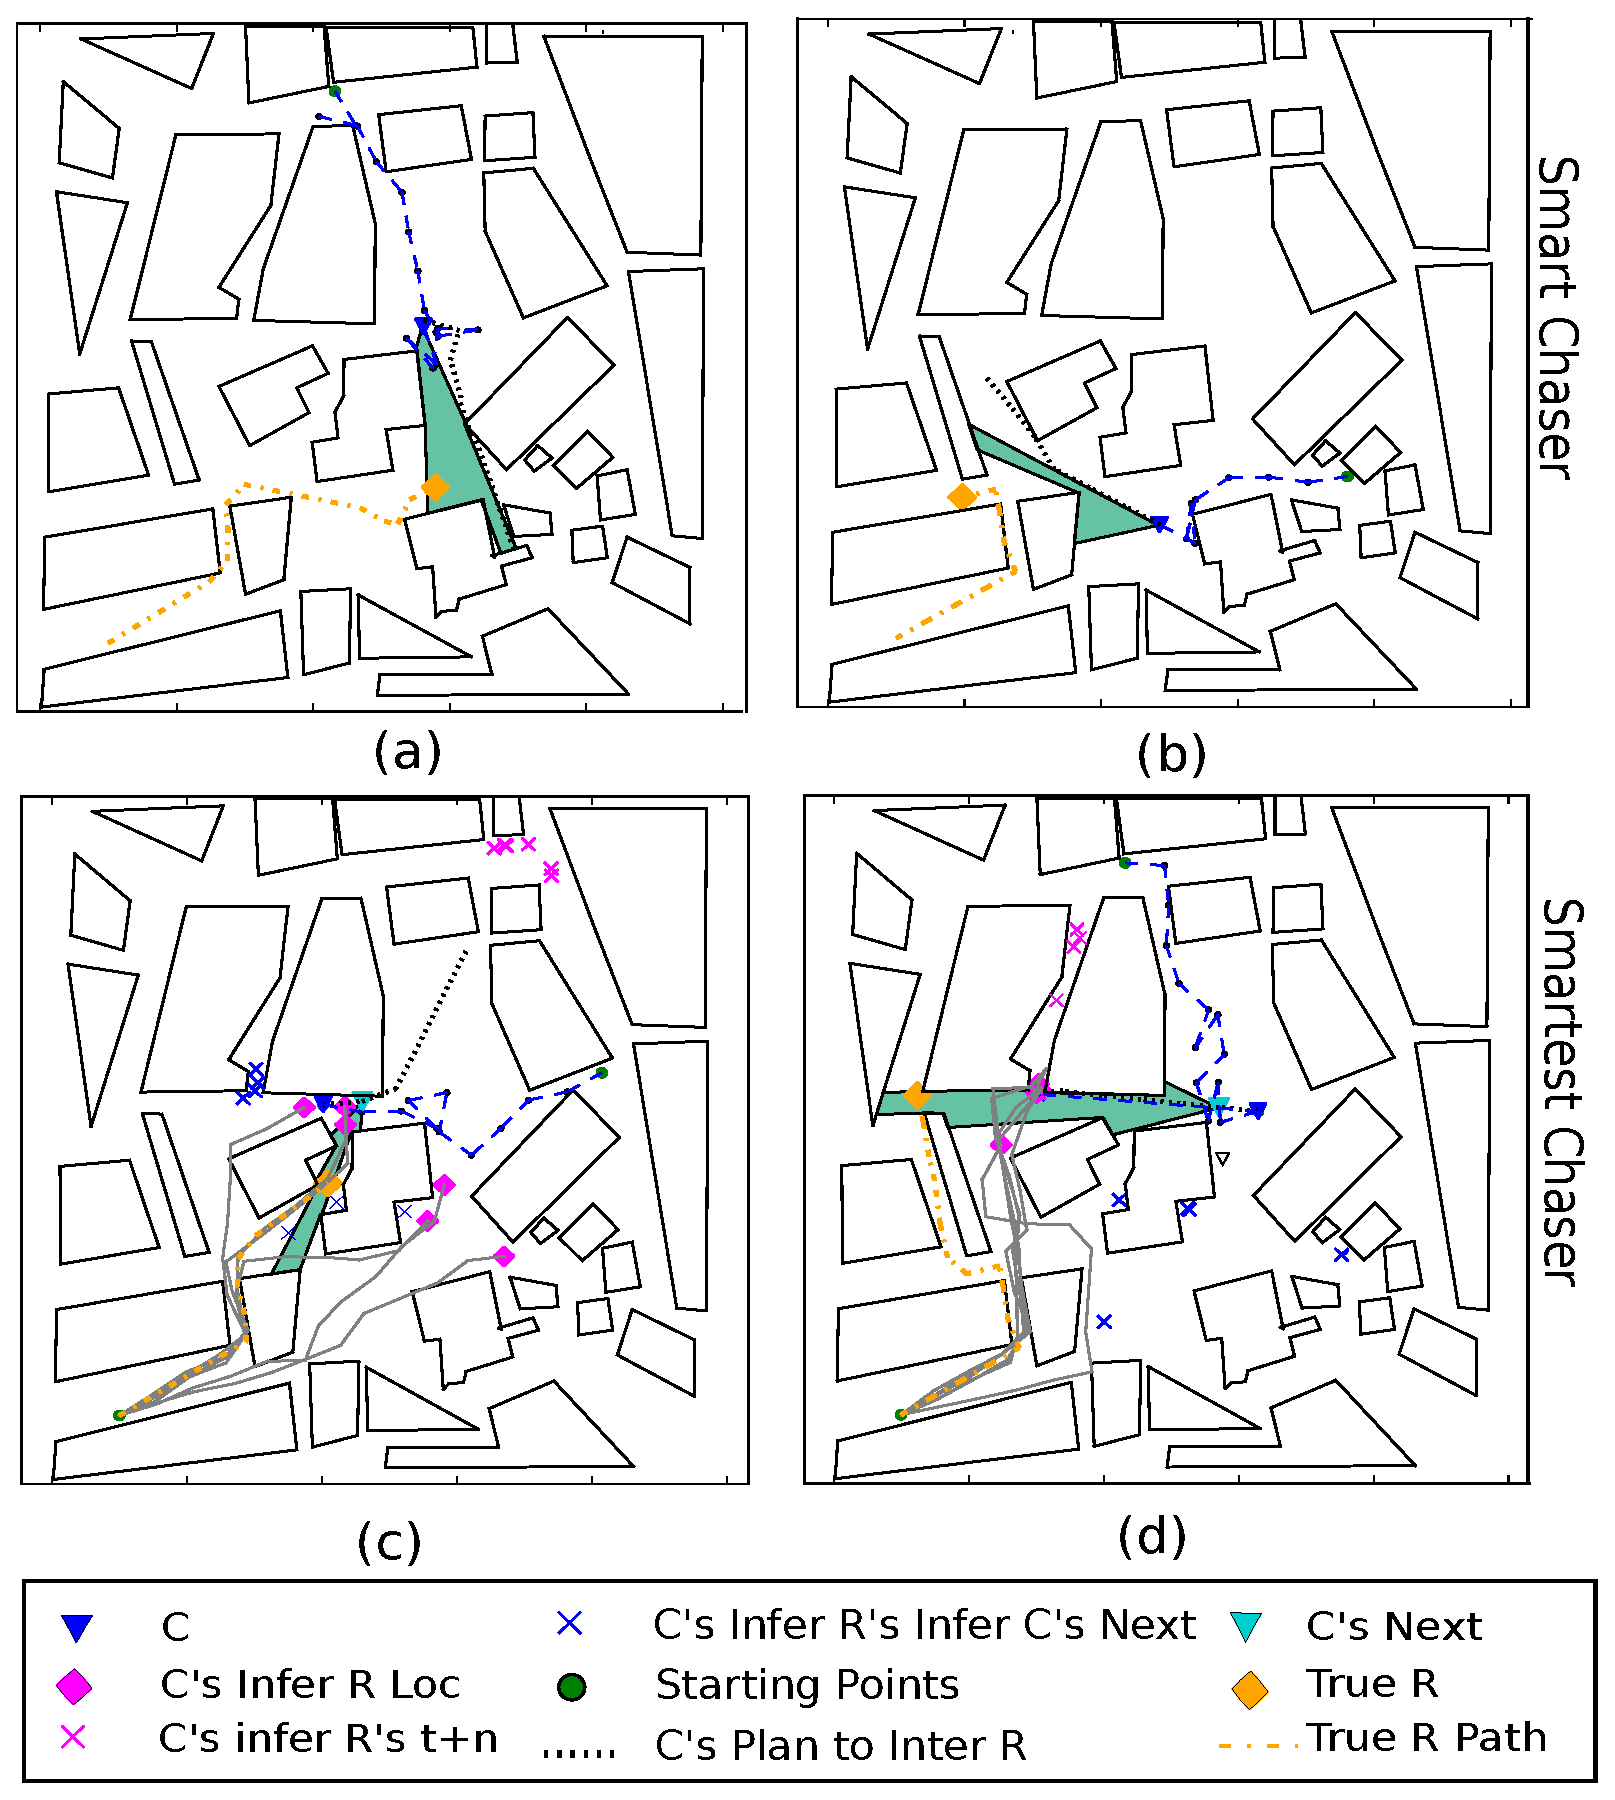
\includegraphics[width=0.9\columnwidth]{detection_examples.eps}}
\caption{(a) Smart chaser playing against a naive runner, where the chaser anticipates the the intersection point and heads in the correct direction to detect the runner. (b) Smart chaser playing against a smarter runner. (c) Smartest chaser against the naive runner. (d) Smartest Chaser infers the runner locations to be more hidden, avoiding the center of the map. The chaser successfully detects the smarter runner. See text for details. }
\label{fig:exps}
\end{center}
\vskip -0.4in
\end{figure} 


%-------------------------


\begin{table}[!b]
\caption{Detection Rates for Types of Agents}
\centering
\begin{tabular}{c"c|c}
    \hline\hline 
    $\ $ & naive runner & smarter runner \\\thickhline
    smart chaser & $(49/50)=0.98$ & $(18/50)=0.36$ \\\hline
    smartest chaser & $(49/50)=0.98$ & $(28/50)=0.56$ \\\hline
\end{tabular}
\label{table:detect_rates}
% \vskip -0.2in
\end{table}


\subsection{Detection Experiments}
\vspace{-0.5em}
For our second set of experiments, we apply our Chaser-Runner model in a couple of scenarios where we compare detection rates against a basic (i.e non-theory-of-mind) chaser model, which we describe later in the section. We run simulations using two types of runners, a \textit{naive runner} which plans from start to goal locations directly with RRT plans, and a \textit{smarter runner} which plans from start to goal locations using a basic runner model to avoid naive path-planning chasers. We show that when the chaser has an accurate model of the runner, the detection rates over episode restarts are relatively high compared to when it has an inaccurate model of the runner. Additionally we show that a more complex chaser model can perform just as well as a basic chaser model when in search of a naive runner and performs better against a smarter runner. 

%  We define a smart chaser that has an accurate mental model of the naive runner by adjusting our Chaser-Runner model (set to $(K,L)=(128, 1)$), to condition only the outer model to maximize its utility. Since we do not condition the middlemost model, the runner is not rewarded for any planning, therefore simulating naive plans.
 
 
\textbf{Experiment #1: Naive Runner, Smart Chaser.} The first experiment illustrates how a relatively \emph{smart chaser} can reliably head off and detect a \emph{naive runner}. We define the naive runner to be a runner that simply plans a path from its start to goal location, without any particular reasoning about the chaser.  %-- in other words, the smart chaser expects the naive runner to plan a path directly from start to goal. 
This setup of our chaser implies that our \textit{smart chaser} will sample plans that tend to head off the naive runner.  
Figure~\ref{fig:exps} (a) illustrates a prototypical result.  
The chaser's plans tend to keep crossing the center of the map where it reliably detects the runner. This experiment is composed of 50 restarts (of the episode), uses the same naive runner in each restart, and results in a detection rate of 0.98, Table~\ref{table:detect_rates}. 

% This experiment had a relatively high detection rate of $\approx 0.80$, shown in Table~\ref{table:detect_rates}.


\textbf{Experiment #2: Smarter Runner, Smart Chaser.} For our second experiment, we increase the model complexity of the runner.  The \emph{smarter runner} is a runner with a mental model of a chaser that has a mental model of a simple runner. The smarter runner expects the chaser to remain in the center of the map, as it is trying to head off a naive agent.

The smart chaser is the same as in Experiment #1.  
Figure~\ref{fig:exps} (b) illustrates a prototypical result.  Because the smarter runner knows how to avoid the chaser, and because the chaser still has a mental model of a runner that goes straight for the goal, the runner avoids detection. In Figure~\ref{fig:exps} (b), the runner is seen swerving sharply left taking a longer path around the perimeter of the city to reach its goal. As a result, the chaser is unable to find the runner for the rest of the simulation. Our experiments, composed of 50 restarts with identical smarter runner trajectories, revealed a lower detection rate of 0.36, shown in Table~\ref{table:detect_rates}.
\vspace{1em}
% % --------------------------------------------------------------------------------

\textbf{Experiment #3: Naive Runner, Smartest Chaser.} In this next experiment, we use the identical naive runner from Experiment #1, but the chaser is the Chaser-Runner model, described in Section~\ref{sec:tcrm}, using $(K,L)=(128, 16)$ with \textbf{both} outer and middlemost models conditioned to maximize utility. In other words, the chaser assumes a non-naive runner, even though the runner's behavior is in fact naive. 

Figure~\ref{fig:exps} (c) illustrates a prototypical result.
This figure is an example of a successful detection.
`C' stands for Chaser; `R' stands for runner.  The
blue triangle represents the chaser's true, current location; blue
dashed lines and Xs represent the chaser's inferences about the
runner's inferences about where the chaser will move next (this is the result of inference in the middlemost model). Magenta diamonds represent samples of where the chaser thinks the runner is;
magenta Xs represent samples of where the chaser thinks the runner
will move next. The chaser correctly predicts the runner's expected
next location (blue circle) and plans a path to intercept it (black
dashed line); the chaser's isovist is shown as a light green
polygon.

Here, the multimodality of the model's inferences is apparent: the chaser predicts two possible modes where the runner could be (clusters of magenta triangles), but assigns more probability mass to the upper (correct) cluster; the result is that the chaser plans a path to that location, which results in a detection. After running 50 restarts, this experiment resulted in a detected rate of 0.98 (shown in Table~\ref{table:detect_rates}), where we us the same previous naive runner as Experiment 1 in each restart.


\begin{figure}[!t]
\begin{center}
\centerline{\hspace{-0.2em}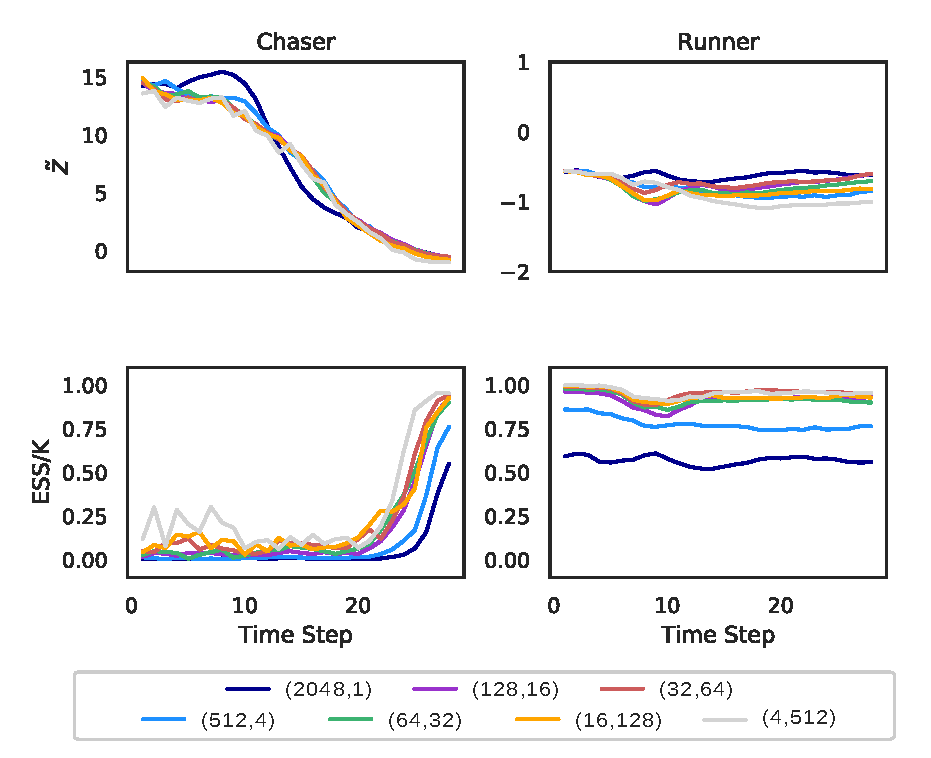
\includegraphics[width=1.05\columnwidth]{EXP-particle_exp_updated_legend.eps}}
\caption{ Log mean log weights, $\tilde{z}$, and Fractional ESS (normalized by $K$) as a Function of Time for each sample budget. \textbf{Top Row:}  $\tilde{z}^\textsc{R}$ for the middlemost model (left), and $\tilde{z}^\textsc{C}$ the outermost model, (right). \textbf{Bottom Row:} The fractional ESS for each varying $K$ and $L$.  }
%Varying sampling sizes for the respective outermost and middlemost model: 2048x1 (dark blue), 512x4 (blue), 128x16 (violet), 64x32 (green), 32x64 (red-brown), 16x128 (orange), 4x512 (light grey).    }
\label{fig:log_means}
% \label{fig:exps}
\end{center}
\vskip -0.4in
\end{figure} 

\textbf{Experiment #4: Smarter Runner, Smartest Chaser.} This experiment tests our fully implemented theory of mind model, the Chaser-Runner model using $(K,L)=(128,16)$ against the smarter runner (used in Experiment 2).  Figure~\ref{fig:exps} (c) illustrates a prototypical result and an example of a successful detection. As seen, the chaser now predicts the runner will avoid highly visible areas of the map and travel through alley ways and around the city. In this scenario, we see that the model's inference become unimodel and the chaser is able to detect the chaser. This experiment yielded a detection rate of 0.56 after running 50 restarts, shown in Table~\ref{table:detect_rates}. Although these detection rates may seem low at first, recall that Experiment 2 yielded a low 0.36 detection rate. By implementing the full theory of mind model, we see that the chaser improves detection rates and is able to successfully model and infer the behavior of the smarter agent.

\textbf{Discussion} Table~\ref{table:detect_rates} collects the detection rates for each of the four experiments.  In Experiment 1, the smart chaser has a correct model of the runner, and therefore has a relatively high detection rate of 0.98. When the naive runner competes against the smartest chaser (Experiment 3), the detection performance is maintained. When the smarter runner is introduced (Experiment 2), detection rates for the smart chaser decrease to 0.36.  Lastly, when we simulate the our nested models, the rates increase to 0.56. 

This strengthens the generally accepted idea that better models matter. When the runner reasons more deeply, he evades more effectively; when the chaser reasons more deeply, he intercepts more effectively. Furthermore, a single, unified inference algorithm results in a wide variety of intuitive, rational behavior for both the runner and the chaser, perhaps suggesting that good models are more important than complex inference algorithms, at least for simple problems.


\subsection{Sample Particle Budget Experiment}
\vskip -0.05in

\begin{figure}[!t]
\begin{center}
\centerline{\hspace{-0.2em}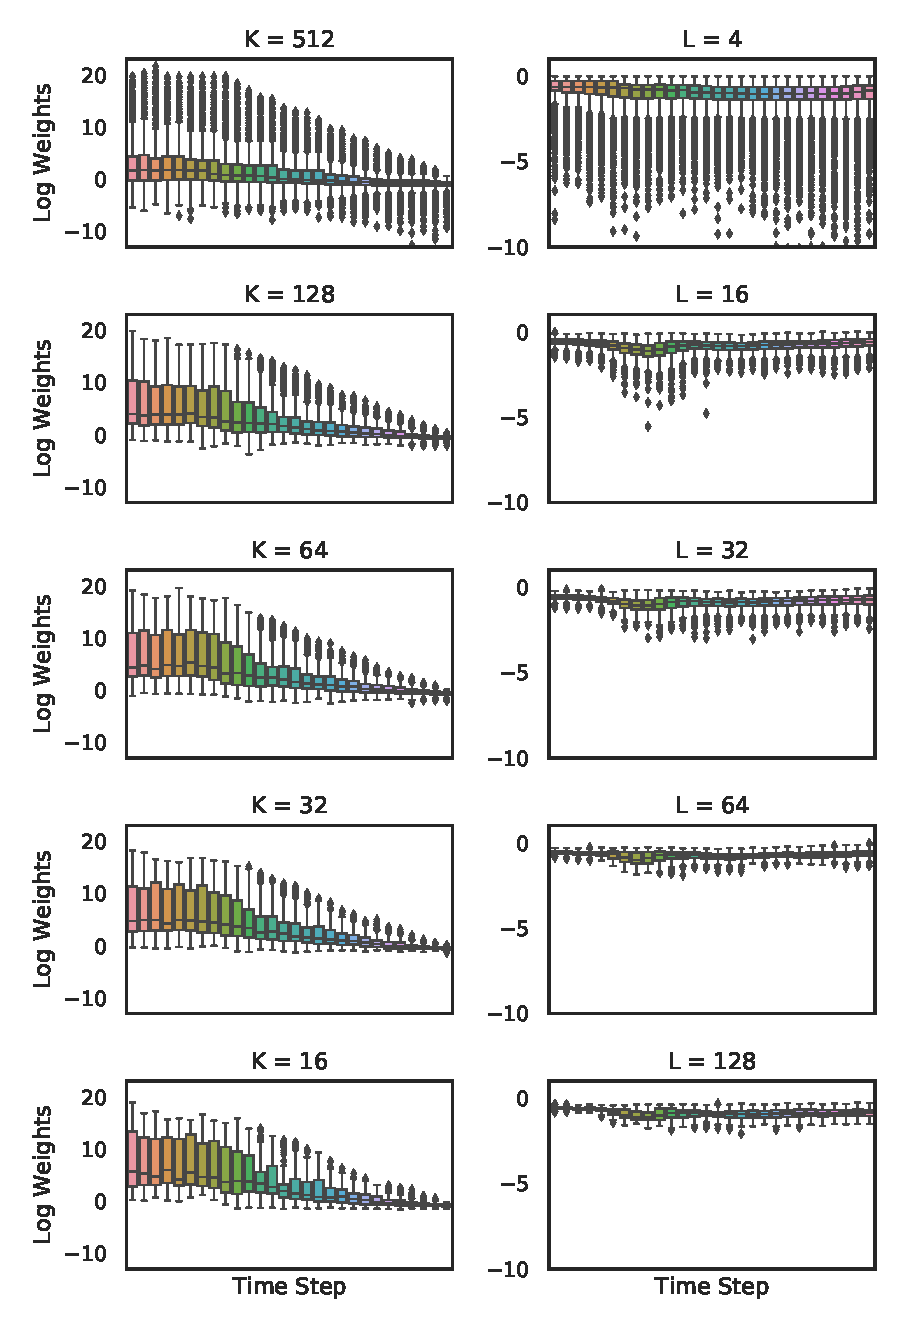
\includegraphics[width=1.05\columnwidth]{EXP-A2-particle_var.eps}}
\caption{Box plots showing quantiles of log weights for the runner (left) and chaser (right) at each time step in the simulation for varying $K$ and $L$.}
\label{fig:box_plots}
%Log weight variance with K=512 L=4, K=128, L=16, and K=16, L=128.}
% \label{fig:exps}
\end{center}
\vskip -0.4in
\end{figure} 

%After running our detection experiments, we asked ourselves, does the number of particles sampled at each level of the model matter? In hind sight, should we have taken into account the difficulty level of sampling effective samples from each model? For example, we could consider a case where we would require a high number of samples from the chaser's runner model due to its difficulty in producing samples with low detection probabilities. On the other hand, we could consider the case where sampling from the chaser's runner model would need only a small sample size due to its ability to produce effective samples easily. We, of course, considered the same cases with the chaser model. 

As a final set of experiments, we quantify how the allocation of our computational budget affects the reliability of our importance sampling estimator. To do so, we vary $K$ and $L$ while keeping the total number of samples fixed at $K \cdot L = 2048$. Given this budget, we vary $K$ and $L$ over the range
\vskip -0.3in
\[
    (K,L) = (2048,1), (512, 4), (128, 16), \ldots (4,512)
\]
\vskip -0.1in
In the model that we defined in Section~\ref{sec:tcrm}, the chaser weights $w^\textsc{c}$ and runner weights $w^\textsc{r}$ reflect the probability of detection from the perspective of the chaser and runner respectively.
%
% Figure 4 TOP ROW
For this experiment, we run $R=10$ independent restarts for each sample budget, $S=7$, resulting in a total of $(S \cdot R \cdot T \cdot K  \cdot L)$ weights, where $T$ denotes the number of time steps for each episode. Since our RRT planner returns a total of 30 steps, $T= 28$ when we exclude corresponding time steps for the start and goal locations. In Figure~\ref{fig:log_means} (top row), for each sample budget, we compute
$\tilde{z}$, the log mean log weights, across ($R \cdot K \cdot L$) for each time step. We show that for each sample budget, $\tilde{z}^\textsc{c}$ decreases (left) as a function of time while $\tilde{z}^\textsc{r}$ remain relatively stable independent of time (right).  It is to be expected that $\tilde{z}^\textsc{c}$ decrease as a function of time given the lower probability of encountering the runner before the episode ends.

% Figure 4 BOTTOM ROW
To get a notion of the weight variance at each time step, we compute the Effective Sample Size, which for a set of $K$ weights $\{w_k\}$ is defined as 
\vskip -0.1in
\[
    \textstyle \text{ESS} = \Big(\sum_k w_k \Big)^2 / \sum_k w_k^2.
\]
%\vskip -0.1in
Figure~\ref{fig:log_means} (bottom row), shows the fractional ESS (normalized by $K$) as a function of time for each sample budget. As the the episode continues, the variance between weights decreases, reflecting that inference becomes relatively easier owing to the previously mentioned conclusion of progressively decreasing runner detection probabilities as we reach the end of the episode.

Figure~\ref{fig:box_plots} shows quantiles for log weights, which further confirms the trend in Figure~\ref{fig:log_means} (top left). We show higher median log weights and lower number of outliers as K decreases and L increases, whereas the $(K,L)=(512,4)$ results show that computed log weights are less robust when we draw a smaller number of samples from the middlemost model. To balance between lower variance estimates and maximizing utility for the chaser we used $(K,L)=(32,64)$ in our experiments. 




% --------------------------------------------------------------------------------
% --------------------------------------------------------------------------------
% --------------------------------------------------------------------------------
\vskip -0.1in
\section{Conclusion and Future Work}
\vskip -0.1in

In the beginning of this paper, we considered the question, ``How do we give autonomous agents the ability to infer the mental state of other agents?'', and more importantly, ``How do we reason about that mental state for decision making and planning?'' 
We have taken a step towards this goal by contributing a model with several novel elements, including complex path planning, visibility and nested planning-as-inference.
We %have also proposed and validated a nested importance sampling approach, and 
have shown how relatively straightforward models of theory of mind can capture a variety of rich behavior, and that probabilistic programming is a natural way to describe those models. 
We experimentally demonstrated that runner detections increase as we increase the complexity of the chaser model, therefore showing that more complex models produce improved behavior, and thus improved detection rates. Additionally we show that nested reasoning results in lower-variance estimates of expected utility.
%Our ultimate goal is to implement these ideas on actual UAVs; the extensive case study in this paper suggests that such a goal is achievable in the near future.

One of the virtues of a Bayesian approach is compositionality.  While
we assumed access to a high-level map, the same framework could be
applied to a joint model that blends high-level reasoning with
low-level perception.  In such models, inferences driven by theory of
mind models could go beyond goals and paths, and could additionally
infer (for example) the existence of objects or other agents seen by
the runner, but not by the chaser.  Such integrated models may
require inference metaprogramming; but how best to make
such models computationally tractable is an open question.



%\bibliographystyle{abbrvnat}
%\bibliography{main}
\printbibliography



\end{document}
